\chapter{Series Numéricas e Integrales Impropias}

\section{Series numéricas}

\begin{defi}[serie!de números reales]
    Una serie de números reales es una pareja de sucesiones de números reales
    $(a_n)_{n \geq 0}$, $(s_n)_{n \geq 0}$, relacionadas por
    \[
        s_n = \sum_{i=0}^{n} a_i.
    \]
    Denominaremmos término $n$-ésimo de la serie al elemento $a_n$ y llamaremos
    suma parcial $n$-ésima de la serie a $s_n$.
\end{defi}
\begin{obs}
    Las sumas parciales definen los términos
    \[
        a_0 = s_0, \qquad a_n = s_n - s_{n-1} \quad (n \geq 1).
    \]
\end{obs}

\begin{defi}[suma!de una serie]
    Llamaremos suma de una serie a
    \[
        s = \lim s_n = \lim\limits_{n \to \infty} \sum_{k=0}^{n} a_i,
    \]
    suponiendo que existe.
\end{defi}
\begin{obs}
    Denotaremos $s = \sum\limits_{n \geq 0} a_n = \sum\limits_{n \geq 0}^{\infty} a_n$.
    Esta misma notación nos servirá para representar la serie.
\end{obs}

\begin{defi}[serie!convergente]\index{serie!de números reales!divergente((tlab))}
\index{serie!de números reales!oscilante((tlab))}
    Diremos que una serie $\sum a_n$ es convergente o divergente si lo es la
    sucesión de sumas parciales,
    \begin{itemize}
        \item Convergente: $\lim s_n \in \real$
        \item Divergente: $\lim s_n = + \infty$ o $\lim s_n = - \infty$
        \item Oscilante: $\nexists \lim s_n$.
    \end{itemize}
\end{defi}

\begin{obs}
    Una serie no tiene por qué comenzar por el índice 0, y por tanto, podemos considerar
    series con términos $a_n$ donde $n \geq n_0$. En tal caso, las sumas parciales son
    $s_n = \sum\limits_{k=n_0}^n a_k$, y la suma (si existe) $\sum\limits_{k=n_0}^{\infty}
    a_n = \lim\limits_{n \to +\infty} \sum\limits_{k=n_0}^n a_k$.
\end{obs}


\begin{defi}[serie!geométrica]
    Sea $r \in \real$. Llamaremos serie geométrica de razón $r$ a la serie
    \[
        \sum_{n \geq 0} r^n.
    \]
\end{defi}

\begin{prop}
    La serie geométrica es convergente si y solo si $\abs{r} < 1$, en tal caso
    la suma es
    \[
        \sum_{n \geq 0} r^n = \frac{1}{1-r}.
    \]
\end{prop}

\begin{proof}
    Primero, calculamos el término $n$-ésimo
    \[
        s_n = 1 + r + \cdots + r^n = \begin{cases}
            n+1 \qquad \text{si } r = 1 \\
            \frac{r^{n+1} - 1 }{r-1} \qquad \text{si } r \neq 1
        \end{cases}
    \]
    \begin{itemize}
        \item Si $r = 1$, $\lim s_n = \lim\limits_{n  \to +\infty} n+1 = +\infty$.
        \item Si $\abs{r} > 1$, $\lim s_n = \lim\limits_{n \to +\infty}
            \frac{r^{n+1} - 1}{r-1} = +\infty$.
        \item Si $\abs{r} < 1$, $\lim s_n = \lim\limits_{n \to +\infty}
            \frac{r^{n+1} - 1}{r-1} = \frac{-1}{r-1}$.
        \item Si $r = -1$, $s_n = 0$ si $n$ par y $s_n = 1$ si $n$ impar. Por
            lo tanto, la serie es oscilante.
    \end{itemize}
\end{proof}

\begin{prop}
    Si $\sum a_n$ es convergente, entonces $\lim a_n = 0$.
\end{prop}

\begin{proof}
    Sabemos que $a_n = s_n - s_{n-1}$, por lo tanto
    $\lim a_n = \lim (s_n - s_{n-1})$, como $\lim s_n$ existe (y por lo tanto
    también $\lim s_{n-1}$)
    \[
        \lim a_n = \lim (s_n - s_{n-1}) = \lim s_n - \lim s_{n-1} = 0.
    \]
\end{proof}

\begin{prop}[Criterio de Cauchy para series]
    La serie $\sum a_n$ es convergente si $\forall\varepsilon>0$,
    $\exists n_0 \in \n$
    tal que
    \[
        m,n \geq n_0 \implies \abs{s_m - s_n} = \abs{a_m + a_{m-1} \cdots + a_n} <
        \varepsilon.
    \]
\end{prop}

\begin{prop}[Linealidad]
    Sean $\alpha, \beta \in \real$ y sean $\sum a_n$ y $\sum b_n$ series convergentes.
    Entonces $\sum (\alpha a_n + \beta b_n)$ también lo es y $\sum (\alpha a_n + \beta b_n)
    = \alpha \sum a_n + \beta \sum b_n$.
\end{prop}

\begin{prop}
    Sean dos sucesiones $(a_n)$ y $(b_n)$, iguales salvo en número finito de términos,
    entonces las series $\sum a_n$ y $\sum b_n$ tienen la misma convergencia.
\end{prop}

\begin{proof}
    Sea $d_n = b_n - a_n$, que vale 0 salvo en número finito de términos
    \begin{itemize}
        \item Si $\sum a_n$ converge, \, $\sum b_n = \sum a_n +
        \overbrace{\sum d_n}^\text{Suma finita}$ $\implies$ $\sum b_n$ converge.
        \item Si $\sum a_n$ diverge, \, $\sum b_n = \sum a_n + \sum d_n
        \implies \sum b_n$ diverge.
        \item Si $\sum a_n$ oscila, \, $\sum b_n = \sum a_n + \sum d_n
        \implies \sum b_n$ oscila.
    \end{itemize}
\end{proof}

\begin{prop}[Asociatividad]
    Sea $\sum a_n$ una serie y $(n_k)_{k \geq 0}$ una sucesión estrictamente creciente de
    números naturales, definimos
    \[
        b_0 = a_0 + \cdots + a_{n_0}, \qquad b_k = a_{(n_{k-1}+1)} + \cdots + a_{n_k}.
    \]
    Si existe la suma de $\sum a_n$, entonces también existe la suma de $\sum b_k$
    y son iguales.
\end{prop}

\begin{proof}
    Sea $A_n = \sum\limits_{i=0}^{n} a_i$ y $B_k = \sum\limits_{i=0}^{k} b_i$, por la
    definición anterior se tiene que $B_k = A_{n_k}$ y por lo tanto $(B_k)$ es una sucesión
    parcial de $(A_n)$, lo cual implica que si $(A_n)$ converge, $(B_k)$ también
    y lo hace al mismo número.
\end{proof}

\section{Series de números positivos}

\begin{prop}
    Si una serie $\sum a_n$ es de \textit{términos positivos} ($a_n \geq 0$) entonces la
    sucesión $(s_n)$ de sumas parciales es \textit{creciente}, y por tanto, siempre tiene
    límite:
    \[
        \sum a_n = \lim s_n = \sup_{n \in \n} s_n.
    \]
    Este puede ser finito (si la sucesión de sumas parciales es acotada) o infinito (en caso
    contrario).
\end{prop}

\begin{prop}[Criterio de comparación directa]
    Sean $\sum a_n$ y $\sum b_n$ series de términos positivos. Si $\exists n_0$ tal que
    $a_n \leq b_n$ ($\forall n \geq n_0$), entonces
    \[
        \sum_{n=n_0}^{\infty} a_n \leq \sum_{n=n_0}^{\infty} b_n.
    \]
    Por tanto, la convergencia de $\sum b_n$ implica la de $\sum a_n$ y la divergencia de
    $\sum a_n$ implica la de $\sum b_n$.
\end{prop}

\begin{proof}
    Por el enunciado
    \[
        \sum_{i=n_0}^{n} a_i \leq \sum_{k=n_0}^{n} b_k \implies
        \sum_{i=n_0}^{\infty} a_i \leq \sum_{k=n_0}^{\infty} b_k.
    \]
    Los términos $a_0, \cdots, a_{n_0}$ se pueden añadir al sumatorio y no alteran
    la convergencia.
\end{proof}

\begin{defi}[serie!harmónica]
    Llamamos serie harmónica a la serie
    \[
        \sum_{n \geq 1} \frac{1}{n}.
    \]
\end{defi}

\begin{defi}[serie!de Riemann]
    Sea $p \in \real$. Llamaremos serie harmónica generalizada o serie de Riemman
    de parámetro $p$ a la serie
    \[
        \sum_{n \geq 1} \frac{1}{n^p}.
    \]
\end{defi}

\begin{prop}
    La serie de Riemman es convergente si y solo si $p > 1$.
\end{prop}

\begin{proof}
    Distinguiremos entre varios casos:
    \begin{itemize}
        \item Si $p = 1$. Suponemos que la serie es convergente con suma $s$
        \[
            s = \left( 1 + \frac{1}{2} \right) + \left( \frac{1}{3} + \frac{1}{4}
            \right) + \cdots > \left( \frac{1}{2} + \frac{1}{2} \right) + \left(
            \frac{1}{4} + \frac{1}{4} \right) + \cdots =
            1 + \frac{1}{2} + \frac{1}{3} + \frac{1}{4} + \cdots = s,
        \]
        contradicción ya que $s>s$.
        \item Si $p < 1$.
        \[
            n^p \leq n \implies \frac{1}{n^p} \geq \frac{1}{n}
        \]
        y por comparación directa con la serie harmónica, diverge.
        \item Si $p > 1$.
        \begin{gather*}
            \sum_{n \geq 1} \frac{1}{n^p} = 1 + \left(\frac{1}{2^p} + \frac{1}{3^p}
            \right) + \left( \frac{1}{4^p} + \frac{1}{5^p} + \frac{1}{6^p} +
            \frac{1}{7^p} \right) + \cdots \leq \\ \leq 1 + \left(\frac{1}{2^p} +
            \frac{1}{2^p} \right) + \left( \frac{1}{4^p} + \frac{1}{4^p} +
            \frac{1}{4^p} + \frac{1}{4^p} \right) = 1 + \frac{1}{2^{p-1}} +
            \frac{1}{2^{2(p-1)}} + \cdots
        \end{gather*}
        que es una serie geométrica de razón $\frac{1}{2^{p-1}} < 1$ y por lo tanto
        convergente.
    \end{itemize}
\end{proof}

\begin{prop}[Criterio de comparación en el límite]
    Sean $\sum a_n$ y $\sum b_n$ series de términos estrictamente positivos.
    Suponemos que existe el límite
    \[
        \lim \frac{a_n}{b_n} = l \in [0,+\infty].
    \]
    \begin{itemize}
        \item Si $l < + \infty$: $\sum b_n$ converge $\implies$ $\sum a_n$ converge y
            $\sum a_n$ diverge $\implies \sum b_n$ diverge.
        \item Si $l > 0$: $\sum a_n$ converge $\implies$ $\sum b_n$ converge y si $\sum b_n$
            diverge $\implies \sum a_n$ diverge.
        \item Si $0 < l < +\infty$: Entonces las dos series tienen el mismo caracter.
    \end{itemize}
\end{prop}
\begin{proof}
    Provaremos cada caso de manera individual
    \begin{itemize}
        \item Caso $l < +\infty$. Fijado $\varepsilon > 0$, por definición de límite, existe
        $n_0\in\n$ tal que
        \[
            n \geq n_0 \implies \frac{a_n}{b_n} < l + \varepsilon \implies
            a_n < (l+\varepsilon)b_n
        \]
        y el resultado queda provado por comparación directa.
        \item Caso $l > 0$. Se deduce del primer caso, considerando
        \[
            \lim \frac{b_n}{a_n} = \frac{1}{l}
        \]
        \item Caso $0 < l < +\infty$. Se trata de una conjunción de los casos
        anteriores
    \end{itemize}
\end{proof}

\begin{lema}
    Sea $\sum a_n$ una serie de términos positivos.
    \begin{itemize}
        \item Suponemos que hay $n_0 \in \n$ y $r < 1$ tal que
        \[
            n \geq n_0 \implies a_n^{1/n} < r,
        \]
        entonces $\sum a_n < +\infty$.
        \item Suponemos que existe $n_0 \in \n$ tal que
        \[
            n \geq n_0 \implies a_n^{1/n} \geq 1,
        \]
        entonces $\sum a_n = +\infty$.
    \end{itemize}
\end{lema}

\begin{proof}
    Provaremos cada caso por separado
    \begin{itemize}
        \item $a_n^{1/n} < r \implies a_n < r^n$ que es la serie geométrica de
        razón $r < 1$, de modo que por comparación directa el resultado queda
        demostrado.
        \item $a_n^{1/n} \geq 1 \implies a_n \geq 1$ y por lo tanto diverge.
    \end{itemize}
\end{proof}

\begin{prop}[Criterio de la raíz de Cauchy]
    Sea $\sum a_n$ una serie de términos positivos. Suponemos que existe
    $\lim a_n^{1/n} = \alpha$, entonces, si $\alpha > 1$ la serie diverge y si
    $\alpha < 1$ la serie converge.
\end{prop}

\begin{proof}
    Demostraremos cada caso por separado
    \begin{itemize}
        \item Caso $\alpha < 1$. Sea $\alpha < r < 1$. Existe $n_0 \in \n$ tal que
        \[
            n \geq n_0 \implies a_n^{1/n} \leq r.
        \]
        El resultado queda provado aplicando el lema anterior.
        \item Caso $\alpha > 1$. Existe $n_0 \in \n$ tal que
        \[
            n \geq n_0 \implies a_n^{1/n} \geq 1,
        \]
        y aplicamos el lema anterior.
    \end{itemize}
\end{proof}

\begin{lema}
    Sea $\sum a_n$ una serie de términos estrictamente positivos.
    \begin{itemize}
        \item Suponemos que hay $n_0 \in \n$ y $r < 1$ tal que
        \[
            n \geq n_0 \implies \frac{a_{n+1}}{a_n} \leq r,
        \]
        entonces $\sum a_n < + \infty$.
        \item Suponemos que existe $n_0 \in \n$ tal que
        \[
            n \geq n_0 \implies \frac{a_{n+1}}{a_n} \geq 1,
        \]
        entonces $\sum a_n = + \infty$.
    \end{itemize}
\end{lema}

\begin{proof}
    Separaremos los casos.
    \begin{itemize}
        \item $\frac{a_{n+1}}{a_n} \leq r$:
        \[
            \frac{a_{n+1}}{a_n} \leq r \implies a_{n+1} \leq r a_n \implies a_n \leq
            C r^n \quad (n \geq n_0)
        \]
        donde $C = \frac{a_{n_0}}{r^{n_0}}$ y, por el criterio de comparación
        directa, $\sum a_n$ converge.
        \item $\frac{a_{n+1}}{a_n} \geq 1$: 
            \[
                \frac{a_{n+1}}{a_n} \geq 1\implies a_{n+1} \geq a_n \implies a_n\text{ es creciente }\implies \sum a_n\text{ diverge}.
            \]
    \end{itemize}
\end{proof}

\begin{prop}[Criterio del cociente de Alembert]
    Sea $\sum a_n$ una serie de términos estrictamente positivos. Suponemos que existe
    $\lim \frac{a_{n+1}}{a_n} = \alpha$, entonces
    \begin{itemize}
        \item Si $\alpha > 1$ la serie diverge.
        \item Si $\alpha < 1$ la serie converge.
    \end{itemize}
\end{prop}

\begin{proof}
    Separamos los dos casos
    \begin{itemize}
        \item Si $\alpha < 1$. Sea $\alpha < r < 1$ entonces $\exists n_0 \in \n$
        tal que
        \[
            n \geq n_0 \implies \frac{a_{n+1}}{a_n} \leq r
        \]
        y aplicamos el lema anterior.
        \item Si $\alpha > 1$. Entonces  $\exists n_0 \in \n$ tal que
        \[
            n \geq n_0 \implies \frac{a_{n+1}}{a_n} \geq 1
        \]
        y aplicamos el lema anterior.
    \end{itemize}
\end{proof}

\begin{example}
    Estudiar la convergencia de
    \begin{itemize}
        \item $\sum\limits_{n \geq 0} \frac{1}{n!}$.
            $n!$ crece más que    $n^2$ ($n! > n^2$) $\implies \frac{1}{n!} < \frac{1}{n^2}$
            que es la serie de Riemman de parámetro 2 (convergente). Por tanto,
            $\sum\limits_{n \geq 0}^\infty \frac{1}{n!}$ es convergente.
        \item $\sum \frac{x^n}{n!}$ para $x > 0$.
            \[
                \lim_{n \to \infty} \frac{\frac{x^{n+1}}{(n+1)!}}{\frac{x^n}{n!}} =
                \lim_{n \to \infty} \frac{x^{n+1}n!}{x^n(n+1)n!} = \lim_{n \to \infty}
                \frac{x}{n+1} = 0 < 1.
            \]
            Por lo tanto, aplicando el criterio del cociente de Alembert, la serie coverge.
        \item $\sum \alpha^{n+\sqrt{n}}$.
            \[
                \lim_{n \to \infty} \alpha^{\frac{n + \sqrt{n}}{n}} =
                \lim_{n \to \infty} \alpha^{1 + \frac{1}{\sqrt{n}}} = \alpha.
            \]
            Por lo tanto, por el criterio de la raíz, $\begin{cases} \alpha < 1
            \text{ convergente} \\ \alpha > 1 \text{ divergente}\end{cases}$. Si $\alpha =1$,
            la serie es $\sum 1^{n + \sqrt{n}} = \sum 1$ que es divergente.
    \end{itemize}
\end{example}

\begin{obs}
    Los criterios anteriores no deciden cuando $\alpha = 1$. Como $\sfrac{a_{n+1}}{a_n} \to
    \alpha$ implica que $a_n^{\sfrac{1}{n}} \to \alpha$, si el criterio del cociente no
    decide, entonces el de la raíz tampoco.
\end{obs}

\begin{prop}[Criterio de Raabe]
    Sea $\sum a_n$ una serie de términos estrictamente positivos tal que existe el límite
    \[
        L = \lim_{n \to \infty} n\left( 1 - \frac{a_{n+1}}{a_n} \right).
    \]
    Si $L > 1$, la serie $\sum a_n$ es convergente. Si $L < 1$, la serie $\sum a_n$ es
    divergente.
\end{prop}

\begin{prop}[Criterio de condensación]
    Sea $(a_n)$ una sucesión de números positivos decreciente, entonces
    \[
        \sum_{n=0}^{\infty} a_n \text{ converge} \iff \sum_{n=0}^{\infty} 2^n a_{2^n}
        \text{ converge}
    \]
\end{prop}

\begin{prop}[Criterio logarítmico]
    Sea $\sum a_n$ una serie de términos positivos tal que existe el límite
    \[
        L = \lim_{n \to \infty} \frac{- \ln(a_n)}{\ln(n)} = \lim_{n \to \infty}
        \frac{\ln\left( \frac{1}{a_n} \right)}{\ln(n)}.
    \]
    Si $L > 1$, la serie $\sum a_n$ es convergente. Si $L < 1$, la serie $\sum a_n$ es
    divergente.
\end{prop}

\begin{prop}[Criterio de la integral]
    Sea $n_0 \in \n$ y $f \colon \left[ n_0, +\infty \right) \to \real$ positiva, localmente integrable
    y decreciente. Consideramos $a_n = f(n)$ ($n \geq n_0$), entonces
    \begin{enumerate}[i)]
        \item La serie $\sum a_n$ y la integral impropia
        $\int_{n_0}^{+\infty} f$ tienen el mismo carácter.
        \item Para $N \geq n_0$
        \[
            \sum_{n \geq n_0}^{\infty} a_n = \sum_{n = n_0}^{N-1} a_n+ \int_{N}^{+\infty}f +
            \varepsilon_N
        \]
        donde $\varepsilon_N \in [0, a_N]$.
    \end{enumerate}
\end{prop}

\begin{example}
    \begin{itemize}
        \item[]
        \item $\sum \frac{1}{n^\alpha}$ tiene el mismo carácter que
            $\int_{1}^{\infty} \frac{1}{x^\alpha} \dif x$ (convergente $\iff \alpha > 1$)
        \item Calcular $\sum\limits_{n\geq 1} \frac{1}{n^{1.01}}$ con error $< 10^{-3}$. \\
            Necesitamos que
            \[
                \frac{1}{N^{1.01}} < 10^{-3} \implies N > 1000^{\sfrac{1}{1.01}} \implies
                N \geq 934
            \]
            Calculamos ahora
            \[
                \sum_{n=1}^{933} \frac{1}{n^{1.01}} + \int_{934}^{+\infty}
                \frac{\dif x}{x^{1.01}} \simeq 100.577 \simeq\sum_{n\geq 1}\frac{1}{n^{1.01}}
            \]
    \end{itemize}
\end{example}

\begin{prop}
    Sea $\sum a_n$ una serie de términos positivos. Dada cualquier permutación $\sigma
    \colon \n \to \n$, la serie $\sum a_{\sigma(n)}$ tiene la misma suma que $\sum a_n$.
\end{prop}

\begin{proof}
    Sea $A_n = \sum\limits_{k=0}^n a_k$ y $B_n = \sum\limits_{k=0}^n a_{\sigma(k)}$ y sean
    $A = \lim A_n$ y $B = \lim B_n$. Sea
    $m \in \n$, entonces $\exists n \in \n$ tal que
    \[
        \setb{0,1, \dots, m} \leq \setb{\sigma(0), \sigma(1), \dots, \sigma(n)},
    \]
    ya que $\sigma$ es suprayectiva. Entonces $a_0 + a_1 + \cdots + a_m \leq a_{\sigma(0)} +
    a_{\sigma(1)} + \cdots + a_{\sigma(n)}$ por lo tanto, $A_m \leq B_n \implies A \leq B$.
    Haciendo el mismo razonamiento para $\inv{\sigma}$ (biyectiva), obtenemos que $B \leq A$.
    Y por lo tanto, $A = \sum a_n = \sum a_{\sigma(n)} = B$.
\end{proof}

\section{Series absoluta y condicionalmente convergentes}

\begin{defi}[serie!absolutamente convergente]
  Diremos que una serie $\sum a_n$ es absolutamente convergente, si la serie $\sum \abs{a_n}$ es convergente.
\end{defi}

\begin{prop}
  Toda serie absolutamente convergente es convergente.
\end{prop}

\begin{proof}
  Aplicamos criterio de Cauchy para series a $\sum \abs{a_n}$: $\forall \varepsilon > 0$ $\exists n_0 \in \n$
  tal que
  \[
    m > n \geq n_0 \implies \abs{\abs{a_{n+1}} + \cdots + \abs{a_m}} < \varepsilon .\implies
    \abs{a_{n+1}} + \cdots + \abs{a_m} < \varepsilon.
  \]
  De donde se deduce que
  \[
    \abs{a_{n+1} + \cdots + a_m} < \abs{a_{n+1}} + \cdots + \abs{a_m} < \varepsilon,
  \]
  por la desigualdad triangular. Y por lo tanto, $\sum a_n$ cumple el criterio de Cauchy.

\end{proof}

\begin{defi}[serie!condicionalmente convergente]
  Una serie convergente, que no es absolutamente convergente, se dice que es condicionalmente convergente.
\end{defi}

\begin{example}
  La serie armónica alternada $\sum \frac{(-1)^n}{n}$ es condicionalmente convergente.
\end{example}

\begin{prop}
    Si $\sum a_n$ y $\sum b_n$ son absolutamente convergentes, y $\lambda \in \real$,
    entonces $\sum (a_n + b_n)$ y $\sum \lambda a_n$ son absolutamente convergentes.
\end{prop}

\begin{defi}[parte!positiva de un real]\index{parte!negativa de un real((tlab))}
  Sea $a \in \real$. Definimos $a_+$ (la parte positiva de $a$) como $a_+ = \max(a, 0)$, asimismo, definimos
  la parte negativa de $a$ como $a_- = \max(-a,0)$.
\end{defi}

\begin{obs}
  Dado un $a$, podemos expresar $a = a_+ - a_-$ y $\abs{a} = a_+ + a_-$.
\end{obs}

\begin{obs}
  Dada $f \colon X \to \real$, podemos hacer exactamente lo mismo, ($f = f_+ - f_-$, $\abs{f} = f_+ + f_-$).
\end{obs}

\begin{example} \hspace{0pt}
  \begin{center}
  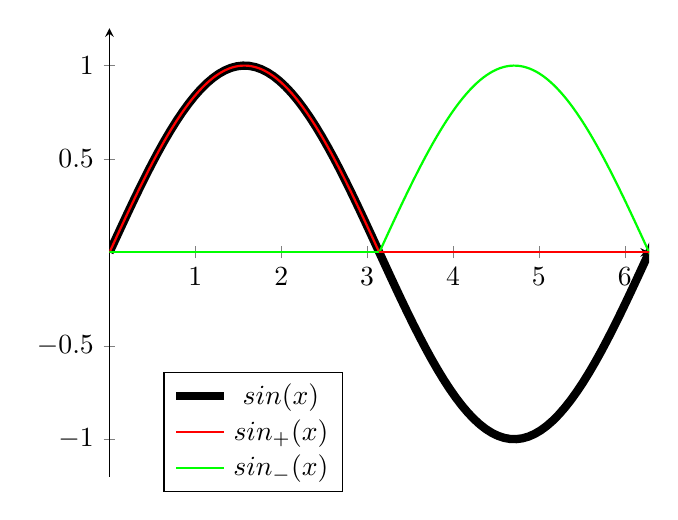
\begin{tikzpicture}
  \begin{axis}[
    xmin = 0,
    xmax = 2*3.14151625,
    ymin = -1.2,
    ymax = 1.2,
    samples = 100,
    axis lines = center,
    legend style={at={(0.1,0.1)},anchor=west}
  ]
    \addplot[domain=0:7,line width=3pt]{sin(deg(x))};
    \addplot[domain=0:3.14151625,color=red,thick]{sin(deg(x))};
    \addplot[domain=3.14151625:7,color=green,thick]{-sin(deg(x))};
    \addplot[domain=3.14151625:7,color=red,thick]{0};
    \addplot[domain=0:3.14151625,color=green,thick]{0};

    \legend{$sin(x)$,$sin_+(x)$,$sin_-(x)$}
  \end{axis}
  \end{tikzpicture}
  \end{center}

\end{example}

\begin{lema}
  Sea $(a_n)$ una sucesión de números reales. Sean $(p_n)$ y $(q_n)$ sus partes positiva y negativa
  (respectivamente),
  \begin{enumerate}[i)]
    \item \label{item:abs_conv_conv}
            $\sum a_n$ converge absolutamente $\iff$ $\sum p_n$, $\sum q_n$ son convergentes.
    \item Si $\sum a_n$ es condicionalmente convergente, entonces $\sum p_n$ y $\sum q_n$ son divergentes.
  \end{enumerate}
\end{lema}

\begin{proof}
  \begin{enumerate}[i)]
      \item[]
      \item Se tiene que
            \[
                \sum\limits_{k=0}^ n \abs{a_k} = \sum\limits_{k=0}^ n p_k + \sum\limits_{k=0}^n q_k.
        \]
        Si $\sum \abs{a_n}$ converge $\implies \sum p_n$ y $\sum q_n$ tienen el mismo carácter,
            como ambas son series de términos positivos, $\sum p_n$ y $\sum q_n$ convergen.

            El recíproco es directo por linealidad.
        \item Se tiene que
            \[
                \sum_{k=0}^n a_k = \sum_{k=0}^n p_k - \sum_{k=0}^n q_k.
            \]
            $\sum p_n$ y $\sum q_n$ no pueden ser las dos convergentes por \ref{item:abs_conv_conv}
            y tampoco puede ser que solo una de las dos sea divergente, porque entonces
            $\sum a_n$ divergería.
  \end{enumerate}
\end{proof}

\begin{prop}
    Si una serie es absolutamente convergente, entonces todas sus series reordenadas
    son convergentes con la misma suma. Es decir, $\forall \sigma \colon \n \to \n$
    permutación, $\sum a_n = \sum a_{\sigma(n)}$.
\end{prop}

\begin{proof}
    Primero, escribimos
    \[
        a_n = p_n - q_n \stackrel{\text{$a_n$ abs. conv.}}{\implies}
        \sum a_n = \sum p_n - \sum q_n.
    \]
    Consideramos ahora $\sigma \colon \n \to \n$ permutación, entonces, $\sum a_{\sigma(n)}$
    también es absolutamente convergente ($\sum \abs{a_{\sigma{n}}} = \sum \abs{a_n}$
    reordenando términos positivos). Ahora tenemos que
    \[
        \sum a_{\sigma(n)} = \sum p_{\sigma(n)} - \sum q_{\sigma(n)}
        \substack{\text{términos} \\ \text{positivos} \\ =} \sum p_n - \sum q_n = \sum a_n.
    \]
\end{proof}

\begin{teo}[de Riemman para series condicionalmente convergentes]
    Sea $\sum a_n$ una serie condicionalmente convergente. $\forall s \in [-\infty,+\infty]$
    existe una reorenación de la serie $\sigma \colon \n \to \n$ (permutación) tal que
    $\sum a_{\sigma(n)} = s$.
\end{teo}

\begin{defi}[serie!alternada]
    Una serie alternada es una serie donde los términos cambian de signo alternativamente.
    Es decir, una serie de la forma $\sum (-1)^n a_n$ donde $a_n \geq 0$.
\end{defi}

\begin{prop}[Criterio de Leibnitz]
    Si $(a_n)$ es una sucesión descendiente de términos positivos con $\lim a_n = 0$,
    entonces  $\sum (-1)^n a_n$ es convergente. Además, si $S_N$ es la $N$-ésima suma
    parcial de $\sum (-1)^n a_n$ y $S$ es su suma, $\abs{S - S_n} \leq a_{n+1}$.
\end{prop}

\begin{proof}
    Consideramos la serie $(S_{2N})$,
    \[
        S_{2N+2} = S_{2N} + \overbrace{(a_{2N+1} + a_{2N+2})}^{\leq 0} \leq S_{2N}.
    \]
    Por lo tanto, $(S_{2N})$ es descendiente, acotada inferiormente por $a_0 - a_1$.
    Consideramos ahora $(S_{2N+1})$,
    \[
        S_{2N+3} = S_{2N+1} + \overbrace{(a_{2N+2} + a_{2N+3})}^{\geq 0} \geq S_{2N+1}.
    \]
    Con lo cual $(S_{2N+1})$ es creciente. Además se tiene que
    \begin{equation}\label{eq:leibn_cotas}
        a_0 - a_1 = S_1 \leq S_{2N+1} \leq S_{2N} \leq S_0 = a_0.
    \end{equation}
    Con lo cual deducimos que tanto $(S_{2N})$ como $(S_{2N+1})$ son convergentes
    (monótonas y acotadas). Por último, tenemos que
    \[
        \lim (S_{2N} - S_{2N-1}) = \lim a_{2N} = 0 \implies \begin{rcases}
            \lim S_{2N} = S \\ \lim S_{2N+1} = S
        \end{rcases} \implies \lim S_N = S.
    \]
    Para acabar, sabemos por (\ref{eq:leibn_cotas}) que S está dentro del intervalo
    de extremos $S_{N}$ y $S_{N+1}$ de longitud $a_{N+1}$, por lo tanto
    $\abs{S - S_N} \leq a_{N+1}$.
\end{proof}

\begin{example}
    La serie harmónica alternada, $\sum \frac{(-1)^n}{n}$ es convergente por el
    criterio de Laibnitz.
\end{example}

\noindent Hay otros criterios de convergencia para series cualesquiera, entre los cuales
destaca el criterio de Dirichlet.

\begin{prop}[Critero de Dirichlet]
    Sean $(a_n)$ y $(b_n)$ dos sucesiones numéricas. Suponemos que
    \begin{enumerate}[i)]
        \item las sumas parciales $s_n$ de la serie $\sum a_n$ están acotadas y
        \item la sucesión $(b_n)$ es positiva y decreciente con límite 0.
    \end{enumerate}
    Entonces la serie $\sum a_nb_n$ es convergente.
\end{prop}

\section{Aplicación: Series de potencias}

\begin{defi}[serie!de potencias]
    Una serie de potencias (centrada en 0) es una expresión
    \[
        \sum_{n \geq 0} a_nx^n,
    \]
    donde $a_n$ son los coeficientes de la serie. A menudo, notaremos simplemente $\sum a_nx^n$.
\end{defi}

\begin{lema}
    El conjunto de los $r \geq 0$ tales
    que $\sum \abs{a_n}r^n$ converge es un intervalo que contiene el 0.
\end{lema}

\begin{proof}
    Si $0 \leq s \leq r$ y $\sum \abs{a_n}r^n$ converge, entonces $\sum \abs{a_n}s^n$
    converge también por comparación directa ($\abs{a_n}s^n \leq \abs{a_n}r^n$) y
    $\sum \abs{a_n}0^n$ converge a 0 trivialmente.
\end{proof}

\begin{defi}[radio de convergencia]\index{dominio de convergencia((tlab))}
    Sea $\sum a_nx^n$ una serie de potencias y sea $I$ el intervalo de los $r \geq$ tales que
    $\sum \abs{a_n}r^n$ converge. Llamamos radio de convergencia de la serie a $R$ el
    extremo superior del intervalo $I$. Denominamos dominio de convergencia de la serie
    al intervalo $(-R,R)$.
\end{defi}

\begin{obs}
    La serie puede converger en los puntos frontera del dominio de convergencia.
\end{obs}

\begin{obs}
    Los casos extremos corresponden a $R = 0$ (la serie solo converge para $x = 0$)
    y $R = +\infty$ (la serie converge para todo $x$).
\end{obs}

\begin{teo}[de Cauchy-Hadamard]
    Sea $\sum a_nx^n$ una serie de potencias. Su radio de convergencia $R$ viene dado por
    \[
        \frac{1}{R} = \limsup \abs{a_n}^{\sfrac{1}{n}}.
    \]
    La serie de potencias es absolutamente convergente si $\abs{x} < R$ y es divergenete
    si $\abs{x} > R$.
\end{teo}

\begin{obs}
    A priori no se puede afirmar nada cuando $\abs{x} = R$.
\end{obs}

\begin{proof}
    Separaremos la demostración en varios casos
    \begin{itemize}
        \item Caso $0 < R < + \infty$. Sea $0 < \abs{x} < R$. Existe $C < 1$ tal que
             \[
                \abs{x} < CR \implies \frac{1}{R} < \frac{C}{\abs{x}}.
            \]
            Por lo tanto, si $n$ es suficientemente grande
            \[
                \abs{a_n}^{\sfrac{1}{n}} \leq \frac{C}{\abs{x}} \implies
                \abs{a_nx^n} \leq C^n.
            \]
            Como $C^n$ es la serie geométrica de razón $C < 1$, la serie converge.

            Sea ahora $\abs{x} > R$, tenemos que $\frac{1}{R} > \frac{1}{\abs{x}}$.
            Hay infinitos $n$ tal que
            \[
                \abs{a_n}^{\sfrac{1}{n}} > \frac{1}{\abs{x}} \implies \abs{a_nx^n} > 1.
            \]
            Por lo tanto $a_nx^n$ no tiende a 0 y por lo tanto la serie no converge.
        \item Caso $R = +\infty$. Entonces $\limsup \abs{a_n}^{\sfrac{1}{n}} = 0$.
            Por lo tanto, para $n$ suficientemente grande $\exists C < 1$ tal que
            $\abs{a_n}^{\sfrac{1}{n}} < \frac{C}{\abs{x}} \implies \abs{a_nx^n} < C^n$ y por lo tanto
            la serie converge.
        \item Caso $R = 0$. Entonces $\forall x$ hay infinitos $n$ tales que
             $\abs{a_n}^{\sfrac{1}{n}} > \frac{1}{\abs{x}} \implies \abs{a_nx^n} > 1 \neq 0$
            y por lo tanto, la serie diverge.
    \end{itemize}
\end{proof}

\begin{obs}
    El radio de convergencia también se puede calcular con las expresiones
    \[
        \frac{1}{R} = \lim \abs{a_n}^{\sfrac{1}{n}} \qquad
        \frac{1}{R} = \lim \frac{\abs{a_{n+1}}}{\abs{a_n}}
    \]
    Suponiendo que los límites existan.
\end{obs}

\begin{example}
    \begin{itemize}
        \item[]
        \item $\sum n!x^n$, $\frac{1}{R} = \lim \frac{(n+1)!}{n!} = \lim (n+1)
            = +\infty \implies R = 0$.
        \item $\sum x^n$, $\frac{1}{R} = \lim 1^{\sfrac{1}{n}} = 1^0 = 1 \implies
            R = 1$.
        \item $\sum \frac{x^n}{n!}$, $\frac{1}{R} = \lim \frac{n!}{(n+1)!} =
            \lim \frac{1}{n+1} = 0 \implies R = +\infty$.
        \item Las series $\sum\limits_{n \geq 0} x^n$, $\sum\limits_{n \geq 1} \frac{x^n}{n}$
            y $\sum \frac{x^n}{n^2}$ tienen $R = 1$, pero tienen comportamiento
            distinto en la frontera.
    \end{itemize}
\end{example}

\begin{defi*}
    Si una serie de potencias $\sum a_n x^n$ tiene radio de convergencia $R > 0$,
    define una función
    \[\begin{aligned}
        f \colon (-R,R) &\to \real \\ x &\mapsto f(x) = \sum a_n x^n
    \end{aligned}\]
\end{defi*}

\begin{obs}
    Se puede probar que $f$ es continua, integrable y derivable
    ``término a término’’.
\end{obs}

\begin{obs}
    La serie derivada término a término tiene radio de convergencia $R$, y por
    lo tanto, la función es de clase $\C^\infty$.
\end{obs}

\begin{proof}
    Primero, consideramos la función derivada $f^\prime (x) = \sum\limits_{n \geq 0}
    n a_n x^{n-1} = \sum\limits_{k \geq 0} (k+1) a_{k+1} x^k$, calculamos ahora
    el radio de convergencia por la definición.
    \[
        \limsup \abs{n+1}^{\sfrac{1}{n}}\abs{a_{n+1}}^{\sfrac{1}{n}} =
        \limsup \abs{n}^{\sfrac{1}{n-1}}\abs{a_{n}}^{\sfrac{1}{n-1}} =
        \limsup \left( n^{\sfrac{1}{n}} \abs{a_n}^{\sfrac{1}{n}} \right)^
        {\frac{n}{n-1}} = \frac{1}{R},
    \]
    además
    \[
        f^{(k)}(0) = k! a_k \rightarrow f(x) = \sum_{k \geq 0} \frac{f^{(k)}(0)}
        {k!}x^k.
    \]
\end{proof}

\begin{defi}[serie!analítica]
    Una función tal que alrededor de cada punto se puede expresar como una serie
    de potencias (convergente) se llama analítica.
\end{defi}

\begin{defi}[serie!de Taylor]
    Sea $D$ un intervalo abierto tal que $0 \in D$ y sea $f \colon D \to \real$
    de clase $\C^\infty$. Entonces, $f$ define una serie de potencias
    \[
        \sum_{n \geq 0} \frac{f^{(n)}(0)}{n!} x^n,
    \]
    que es la serie de Taylor de $f$ (centrada en 0).
\end{defi}

\begin{prop}
    Sea $D$ un intervalo abierto tal que $0 \in D$ y sea $f \colon D \to \real$
    de clase $\C^\infty$. Suponemos que la serie de Taylor de $f$ tiene radio
    de convergencia $R > 0$. Recordando la fórmula de Taylor $f(x) = P_n(x) + R_n(x)$
    (donde $P_n$ es el polinomio de Taylor de grado $\leq n$ de $f$ en 0, y $R_n$
    el correspondiente residuo de Taylor), por tanto en $D \cap (-R,R)$,
    \[
        f(x) = \sum_{n \geq 0} \frac{f^{(n)}(0)}{n!}x^n \iff
        \lim_{n \to \infty} R_n(x) = 0.
    \]
\end{prop}

\begin{obs}
    Hay funciones $f \colon \real \to \real$ de clase $\C^\infty$ tales que su
    serie de Taylor (centrada en 0) converge para todo $x$, pero no coincide con
    $f(x)$ en ningún punto salvo el origen. \\
    Hay funciones $f \colon \real \to \real$ de clase $\C^\infty$ tales que su
    serie de Taylor (centrada en 0) tiene radio de convergencia 0.
\end{obs}

\begin{example}
    La función $f(x) = \begin{cases} 0 \quad \text{si } x \leq 0 \\
    e^{-\sfrac{1}{x^2}} \quad \text{si } x > 0 \end{cases}$
    \begin{center}
    \begin{tikzpicture}
    \begin{axis}[
        xmin = -1,
        xmax = 2,
        ymin = -1.2,
        ymax = 1.2,
        samples = 100,
        axis lines = center
    ]
        \addplot[domain=-1:0,color=blue,thick]{0};
        \addplot[domain=0:2,color=blue,thick]{e^(-1/x)};
    \end{axis}
    \end{tikzpicture}
    \end{center}
    Su serie de Taylor es nula ($f^{(k)}(0) = 0$ $\forall k \in \n$). Pero $f$ no
    se anula en ningún entorno de 0 $\implies$ $f$ no coincide con la serie de
    Taylor en ningún entorno de 0.
\end{example}

\begin{prop}[Algunas series de Taylor importantes]
    \begin{itemize}
        \item[]
        \item $\displaystyle e^x = \sum_{n \geq 0} \frac{x^n}{n!}
            \qquad \forall x \in \real$.
        \item $\displaystyle \cos(x) = \sum_{n \geq 0} (-1)^{n}\frac{x^{2n}}{(2n)!}
            \qquad \forall x \in \real$.
        \item $\displaystyle \sin(x) = \sum_{n \geq 0} (-1)^{n}\frac{x^{2n+1}}{(2n+1)!}
            \qquad \forall x \in \real$.
        \item $\displaystyle \log(1+x) = \sum_{n \geq 1} (-1)^{n+1} \frac{x^n}{n}
            \qquad \abs{x} < 1$.
        \item $\displaystyle (1+x)^p = \sum_{n \geq 0} {p \choose n} x^n \qquad
            \begin{cases} x \in \real \quad \text{si } p \in \n \\ \abs{x} < 1
            \quad \text{si } p \notin \n \end{cases}$.
        \item $\displaystyle (1+x)^{-1} = \sum_{n \geq 0} (-1)^n x^n \qquad \abs{x} < 1$.
    \end{itemize}
\end{prop}

\begin{example}
    \begin{itemize}
        \item[]
        \item $\displaystyle \sum_{n \geq 0} \frac{1}{n!} = e^1 = e$.
        \item $\displaystyle \frac{1}{(1-x)} = \sum_{n \geq 0} x^n \implies
            \sum_{n \geq 1} n x^{n-1} = \left( \frac{1}{(1-x)} \right)' =
            \frac{1}{(1-x)^2}$.

            Por lo tanto
            \[
                \sum_{n \geq 1} nx^n = \frac{x}{(1-x)^2}.
            \]
        \item $f = \arctan(x)$ con $\abs{x} < 1$ (a partir de $f'(x) = \frac{1}{1+x^2}$)
            \[
                \frac{1}{1+x^2} = \sum_{n \geq 0} (-1)^n x^{2n} \implies
                \arctan(x) = \int \frac{1}{1+x^2} \dif x = \sum_{n \geq 0} (-1)^n
                \frac{x^{2n+1}}{2n+1}.
            \]
    \end{itemize}
\end{example}

\subsection{Series de números complejos}

\begin{defi*}
    La definición de serie, de serie convergente y de serie absolutamente convergente,
    es la misma si, en vez de considerar números reales, consideramos números
    complejos.
\end{defi*}

\begin{prop}
    Una serie $\sum c_n$ de números complejos es convergente si y solo si lo son
    separadamente sus partes real e imaginaria.
\end{prop}

\begin{prop}
    Toda serie $\sum c_n$ de números complejos absolutamente convegente, es
    convergente.
\end{prop}

\begin{obs}
    El estudio de las series de potencias es completamente análogo. En el caso
    complejo, si la serie de potencias $\sum c_n z^n$ tiene radio de convergencia
    $R$ ($\frac{1}{R} = \limsup \abs{c_n}^{\sfrac{1}{n}}$). Entonces, el dominio de
    convergencia es un disco abierto $\abs{z} < R$ del plano complejo.
\end{obs}

\begin{obs}
    La serie de Taylor de la función exponencial real permite definir la exponencial
    compleja como
    \[
        e^z = \sum_{n \geq 0} \frac{z^n}{n!}, \forall z \in \cx.
    \]
\end{obs}

\begin{prop}
    Tomando $z \in \cx$ un imaginario puro, y separando las partes real e imaginaria
    de las potencias, obtenemos la formula de Euler,
    \[
        e^{ix} = \cos(x) + i\sin(x).
    \]
    En particular para $x = \pi$, se tiene que $e^{i\pi} + 1 = 0$.
\end{prop}



\section{Integrales impropias: definición y ejemplos}

\begin{defi}[función!localmente integrable]
    Sea $D \subset \real$ un intervalo, y $f \colon D \to \real$ una función.
    Diremos que $f$ es localmente integrable si es integrable para todo intervalo
    compacto $K \subset D$.
\end{defi}
\begin{obs}
    Si consideramos por ejemplo, $f \colon [a,b) \to \real$ con $a < b \leq +\infty$.
    Entonces, $f$ es localmente integrable si es integrable en cualquier intervalo
    $[a,M]$ donde $a < M < b$. \\
    En tal caso, podemos estudiar la integral impropia
    \[
        \int_a^b f := \lim_{M \to b^-} \int^M_a f.
    \]
\end{obs}

\begin{obs}
    A veces se dice que una integral impropia es
    \begin{itemize}
        \item De primera especie, si el intervalo no es acotado.
        \item De segunda especie, si la función no es acotada.
        \item De tercera especie, sin ni la función ni el intervalo son acotados.
    \end{itemize}
\end{obs}

\begin{defi}[integral!impropia!convergente]\index{integral!impropia!divergente((tlab))}
    Diremos que la integral impropia es convergente si $\exists\abs{\int^b_a f}
    <+\infty$, y divergente si $\exists\int^b_a f = \pm\infty$.
\end{defi}

\begin{obs}
    De forma totalmente análoga, podemos considerar la integral impropia de una
    función $f \colon (a,b] \to \real$ localmente integrable, con $-\infty \leq a
    < b$.
\end{obs}

\begin{defi}[integral!impropia]
    Consideramos una función localmente integrable $f \colon (a,b) \to \real$. Si
    tomamos un punto arbitrario $c$ tal que $a < c < b$, podemos descomponer
    \[
        \int^b_a f := \int^c_a f + \int^b_c f = \lim_{M \to a^+} \int^c_M +
        \lim_{N \to b^-} \int^N_c f
    \]
    y estudiar las dos integrales impropias. Si las dos son convergentes, una
    es convergente y la otra divergente o las dos son divergentes con el mismo
    signo, entonces se define la integral impropia del primer miembro como la
    suma de las dos del segundo miembro.
\end{defi}
\begin{obs}
    Más generalmente, podemos considerar una función localmente integrable definida
    en un dominio $D$ que sea unión finita y disjunta de intervalos. Entonces,
    definimos $\int_D f$ como la suma de las integrales sobre estos intervalos,
    suponiendo que sean convergentes.
\end{obs}

\begin{prop}
    Consideramos una función integrable por Riemman, $f \colon [a,b] \to \real$,
    entonces
    \[
        \int^a_b f = \lim_{M \to b^-} \int^M_a f.
    \]
\end{prop}

\begin{obs}
    Así, la notación introducida para las integrales impropias no produce ningún
    conflicto con la notación habitual definida para integrales ``propias’’.
\end{obs}

\begin{example}
    Algunos ejemplos de integrales importantes son
    \begin{itemize}
        \item $\displaystyle \int^{+\infty}_1 \frac{\dif x}{x^\alpha}$. Es
            convergente si y solo si $\alpha > 1$ $\left(\text{y vale }
            \frac{1}{\alpha-1}\right)$. Y es divergente si $\alpha \leq 1$.
            \[
                \lim_{M \to +\infty} \int^M_1 \frac{\dif x}{x^\alpha} =
                \begin{cases}
                    \alpha = 1 \quad \lim\limits_{M \to +\infty}
                    \left[\log x \right]^M_1 = + \infty \\
                    \alpha \neq 1 \quad \lim\limits_{M \to +\infty}
                    \left[\frac{x^{-\alpha+1}}{-\alpha+1}
                    \right]^M_1 = \lim\limits_{M \to +\infty}
                    \frac{M^{-\alpha+1}-1}{-\alpha+1}=\begin{cases}
                        \frac{1}{\alpha-1} \quad
                        \text{si $\alpha > 1$} \\
                        +\infty \quad \text{si $\alpha < 1$}
                    \end{cases}
                \end{cases}
            \]
        \item $\displaystyle \int^1_0 \frac{\dif x}{x^\alpha}$. Es convergente
            si y solo si $\alpha < 1$ $\left(\text{y vale } \frac{1}{1-\alpha
            }\right)$. Y es divergente si $\alpha \geq 1$.

            Podemos observar que
            \[
                \int^{+\infty}_0 \frac{\dif x}{x^\alpha} = \int^1_0
                \frac{\dif x}{x^\alpha} + \int^{+\infty}_1
                \frac{\dif x}{x^\alpha} = +\infty,
            \]
            independientemente del valor de $\alpha$.
        \item $\displaystyle  \int^{+\infty}_0 e^{-ax} \dif x$. Es convergente
            si y solo si $\alpha > 0$ $\left(\text{y vale }\frac{1}{\alpha}\right)$.
    \end{itemize}
\end{example}

\begin{example}
    \begin{itemize}
        \item[]
        \item $\int^{+\infty}_0 \frac{\dif x}{1+x^2}$
            \[
                \int^{+\infty}_0 \frac{\dif x}{1+x^2} =
                \lim_{M \to +\infty} \left[\arctan x\right]^M_0 =
                \frac{\pi}{2}
            \]
            \[
                \int^{+\infty}_{-\infty} \frac{\dif x}{1+x^2} =
                \int^0_{-\infty} \frac{\dif x}{1+x^2} +
                \int^{+\infty}_0 \frac{\dif x}{1+x^2} = \pi.
            \]
        \item $\int^1_{-1} \frac{\dif x}{x^2}$
            \[
                \int^1_{-1} \frac{\dif x}{x^2} = \int^0_{-1}
                \frac{\dif x}{x^2} + \int^1_0 \frac{\dif x}{x^2} =
                +\infty.
            \]
            Pero $\left[-\frac{1}{x}\right]^1_{-1} = -2$, es decir, que no
            podemos aplicar la regla de Barrow.
        \item $\displaystyle \int^{+\infty}_{-\infty} x\dif x$: No existe
        \item $\int^1_0 \frac{1}{x^2}\cos x \dif x$
            \[
                \int^1_0 \frac{1}{x^2}\cos x \dif x =
                \left[ \cos \frac{1}{x} \right]^1_0 = \cdots
                \text{ No existe.}
            \]
    \end{itemize}
\end{example}

\begin{obs}
    Las reglas de cálculo de integrales se aplican a las integrales impropias
    teniendo en cuenta que hay que aplicar un límite. Explicitamos algunas.
\end{obs}

\begin{prop}[Linealidad]
    Si $\int^b_a f$, $\int^b_a g$ son integrales impropias convergentes, tambi\'en
    lo es $\int^b_a (f+g) = \int^b_a f + \int^b_a g$.
    \\
    Si $\int^b_a f$ es convergente y $\lambda \in \real$ $\int^b_a \lambda f =
    \lambda \int^b_a f$.
\end{prop}

\begin{prop}[Regla de Barrow]
    Si $f$ es continua y $f = F^\prime$ en $[a,b)$, entonces
    \[
        \int^b_a f = \lim_{M \to b} F(M) - F(a),
    \]
    suponiendo que el límite exista.
\end{prop}

\begin{prop}[Integración por partes]
    Suponemos que $f,g$ son funciones de clase $\C^1$ en $[a,b)$. Entonces
    \[
        \int^b_a f^\prime g = \lim_{t \to b} \left[ f(x)g(x)\right]^{x=t}_{x=a}
        - \int^b_a g^\prime f,
    \]
    suponiendo que los miembros del segundo t\'ermino existan.
\end{prop}



\section{Criterios de convergencia de integrales impropias}

\begin{prop}[Criterio de Cauchy para integrales impropias]
    Sea $f \colon [a,b) \to \real$ una función localmente integrable. La integral
    impropia $\int^b_a f$ es convergente si y solo si $\forall \varepsilon > 0$ $\exists c_0
    \in [a,b)$ tal que
    \[
        c_0 \leq c_1 < c_2 < b \implies \abs{\int^{c_2}_{c_1} f} < \varepsilon.
    \]
\end{prop}
\begin{proof}
Es consecuencia del criterio de Cauchy aplicado a la función
    \[\begin{aligned}
        F \colon [a,b) &\to \real \\
        x &\mapsto F(x) = \int^x_a f
    \end{aligned}\]
    y el límite $\lim\limits_{x \to b^-}F(x)$ existe si y solo si para todo $\varepsilon >0$
    existe $c_0$ tal que
    \[
        a \leq c_0 \leq c_1 < c_2 < b \implies\abs{F(c_2)-F(c_1)} =
        \abs{\int^{c_2}_{c_1} f} < \varepsilon.
    \]
\end{proof}

\begin{defi}[integral!impropia!absolutamente convergente]
    Diremos que una integral impropia $\int^b_a f$ es absolutamente convergente,
    si la integral impropia $\int^b_a \abs{f}$ es convergente.
\end{defi}

\begin{prop}
    Si $\int^b_a f$ es absolutamente convergente, es convergente.
\end{prop}
\begin{proof}
    Aplicamos el criterio de Cauchy a $\int^b_a \abs{f}$. $\forall \varepsilon >0$,
    $\exists  c_0 \geq a$ tal que $c_0 \leq c_1 < c_2 < b \implies
    \abs{\int^b_a \abs{f}} = \int^b_a \abs{f} < \varepsilon$ y utilizando que 
    $\abs{\int^b_a f} \leq \int^b_a \abs{f}$, tenemos que
    \[
        \abs{\int^b_a f} \leq \int^b_a \abs{f} < \varepsilon.
    \]
    Y por lo tanto, $\int^b_a f$ tambi\'en satisface el criterio de Cauchy, y por
    lo tanto, es convergente.
\end{proof}

\begin{defi}[integral!impropia!condicionalmente convergente]
    Una integral impropia convergente pero no absolutamente convegente, diremos que
    es condicionalmente convergente.
\end{defi}

\begin{prop}
    Sea $f \colon [a,b) \to \real$ (con $a < b \leq +\infty$) localmente integrable
    y positiva ($f \geq 0$), entonces, la función
    \[
        F(x) = \int^x_a f
    \]
    es creciente, y por lo tanto, siempre existe el límite
    \[
        \lim_{x \to b} F(x) = \sup_{x \geq a} F(x).
    \]
    Si $F$ es acotada, entonces la integral imporopia $\int^b_a f$ es convergente,
    en caso contrario, es divergente.
\end{prop}

\begin{prop}[Criterio de comparación directa]
    Sean $f,g \colon [a,b) \to \real$ funciones positivas y localmente integrables.
    Si $f \leq g$, entonces
    \[
        \int^b_a f \leq \int^b_a g.
    \]
    Por lo tanto, si la segunda converge, la primera tambi\'en y si la primera 
    diverge, la segunda tambi\'en.
\end{prop}
\begin{proof}
    \[
        f \leq g \substack{\text{Cálculo I} \\ \implies}
        \int^x_a f \leq \int^x_a g \implies \lim_{x \to b} \int^x_a f \leq
        \lim_{x \to b} \int^x_a g \implies \int^b_a f \leq \int^b_a g.
    \]
\end{proof}

\begin{prop}[Criterio de comparación en el límite]
    Sean $f,g \colon [a,b) \to \real$ estrictamente positivas y localmente
    integrables. Suponemos que existe el límite
    \[
        \lim_{x \to b^-} \frac{f(x)}{g(x)} = L \in [0,+\infty].
    \]
    Entonces, \begin{enumerate}[i)]
        \item\label{item:comp_lim_int_1}
            Si $L < +\infty$, si $\int^b_a g < +\infty \implies \int^b_af <
            +\infty$ $\left( \int^b_a f = +\infty \implies \int^b_a g =
            +\infty\right)$
        \item\label{item:comp_lim_int_2}
            Si $L > 0$, si $\int^b_a f < +\infty \implies \int^b_a g <
            +\infty$ $\left(\int^b_a g = +\infty \implies \int^b_a f =
            +\infty\right)$
        \item Si $0 < L < +\infty$, ambas integrales tienen el mismo carácter.
    \end{enumerate}
\end{prop}
\pagebreak                                  % TODO OJU amb aquesta cutrada
\begin{proof}
    \begin{enumerate}[i)]
        \item[]
        \item Fijada $\varepsilon > 0$, existe $x_0$ con $a < x_0 < b$ tal que
            \[
                x_0 \leq x < b \implies \frac{f(x)}{g(x)} < L +
                \varepsilon \implies f(x) < (L+\varepsilon)g(x).
            \]
            Y aplicamos comparación directa.
        \item Consideramos
            \[
                \lim_{x \to b^-} \frac{g(x)}{f(x)} = \lim_{x \to b^-}
                \frac{1}{\frac{f(x)}{g(x)}} = \frac{1}{L} < +\infty.
            \]
            Por álgebra de límites. Ahora, aplicamos
            \ref{item:comp_lim_int_1}.
        \item Es consecuencia directa de \ref{item:comp_lim_int_1} y de
            \ref{item:comp_lim_int_2}.
    \end{enumerate}
\end{proof}

\begin{prop}[Criterio de Dirichlet]
    Sean $f,g \colon [a,b) \to \real$ funciones localmente integrables. Suponemos
    que
    \begin{itemize}
        \item hay una constante $M > 0$ tal que, si $a < c < b$,
            $\abs{\int^c_a f} < M$ y
        \item $g$ es decreciente con $\lim\limits_{x \to b} g(x) = 0$.
    \end{itemize}
    Entonces, la integral impropia $\int^b_a f(x)g(x)\dif x$ es convergente.
\end{prop}

\begin{example}
    \begin{itemize}
        \item[]
        \item $\int^{+\infty}_{-\infty} e^{-x^2} \dif x = 2
                \int^{+\infty}_0 e^{-x^2} < +\infty$, ya que 
            \[
                e^{-x^2} \leq e^{-x} \implies \int^{+\infty}_1 e^{-x}
                \dif x < +\infty \implies \int^{+\infty}_1 e^{-x^2}
                \dif x < +\infty
            \]
        \item $\int^{+\infty}_1 \left( 1 - \cos \frac{1}{x} \right)
                \dif x < +\infty$, ya que
            \[
                \cos z = 1 - \frac{z^2}{2} + o(z^3) \implies
                1-\cos z \sim \frac{z^2}{2} \implies
                1-\cos \frac{1}{x} \sim \frac{1}{2x^2}.
            \]
            Por lo tanto, $1-\cos \frac{1}{x}$ y $\frac{1}{2x^2}$ son 
            infinitesimos equivalentes, es decir,
            \[
                \lim_{x \to \infty} \frac{1-\cos \frac{1}{x}}
                {\frac{1}{2x^2}} = 1.
            \]
            Como sabemos que $\huge\int^{+\infty}_1 \frac{\dif x}{x^2} <
            +\infty$, aplicamos comparación en el límite.
    \end{itemize}
\end{example}

\begin{example}
    La integral impropia $\int^{+\infty}_0 \frac{\sin x}{x} \dif x$ es
    condicionalmente convergente. \\
    Primero, observamos que la función es el seno cardinal
    \[
        \sinc x = \begin{cases} \frac{\sin x}{x} \quad \text{si } x \neq 0 \\
            1 \quad \text{si } x = 0 \end{cases}
    \]
    que es de clase $\C^{\infty}$, por lo tanto, la integral es de primera especie
    (es impropia por el intervalo). Por lo tanto, podemos estudiar la integral
    $\int^{+\infty}_1 \frac{\sin x}{x} \dif x$ que tendrá el mismo carácter que
    la original. \\
    Vemos que es convergente.
    \[
        \int^{+\infty}_1 \frac{\sin x}{x}\dif x =
        \left[-\frac{\cos x}{x}\right]^{+\infty}_1 - \int^{+\infty}_1 
        -\frac{\cos x}{x^2} \dif x.
    \]
    Ahora observamos que el primero de los sumandos vale $\cos(1)$ y el segundo
    sumando, es absolutamente convergente porque
    \[
        \frac{\abs{\cos x}}{x^2} \leq \frac{1}{x^2} \quad \text{y} \quad
        \int^{+\infty}_0 \frac{\dif x}{x^2} < +\infty.
    \]
    Ahora, veremos que $\int^{+\infty}_1 \frac{\abs{\sin x}}{x}$ es divergente.
    Primero, tenemos que $\frac{\sin^2 x}{x} < \frac{\abs{\sin x}}{x}$ y, tambi\'en
    \begin{gather*}
        \int^{+\infty}_1 \frac{\sin^2 x}{x} \dif x = \int^{+\infty}_1
        \frac{1 - \cos(2x)}{2} \frac{1}{x} \dif x = 
        \left[ \frac{x - \frac{1}{2}\sin(2x)}{2}\frac{1}{x} \right]^{+\infty}_1
        + \int^{+\infty}_1 \frac{x -\frac{1}{2}\sin(2x)}{2}\frac{1}{x^2}\dif x=
        \\ = \frac{1}{2} - \frac{1}{2} + \frac{\sin 2}{4} +
        \frac{1}{2}\int^{+\infty}_{1} \frac{\dif x}{x} + \frac{1}{4}
        \int^{+\infty}_1 \frac{\sin(2x)}{x^2} \dif x = +\infty.
    \end{gather*}
    Ya que la segunda integral es absolutamente convergente (por la misma razón que
    lo era $\int^{+\infty}_1 \frac{\cos x}{x^2}$).
\end{example}
